\chapter{Introduction}\label{chap:introduction}
The proposed project is a multi-project involving all students of the 6th Software semester. The overall purpose of the project, called GIRAF, is to create a set of applications for the Android platform, designed to help people suffering from autism spectrum disorder and their guardians throughout their day. Examples of this are applications like Stemmespillet, which helps people control voice level, and PiktoOplæser which helps them communicate through pictograms and audio.
Previous Software 6 students have also worked on the GIRAF multi-project, the logo of which can be seen in figure \ref{fig:GIRAFlogo}. This means that from the beginning of the semester there was an existing codebase to work on. While previous students have developed several applications, none of them was in a state where they were ready for release. In general, most applications had crash issues and were missing a required connection to the designed database. Some applications were missing features or had implemented some bad workarounds to make them run. It was decided that the focus of this semester should be to refactor and rework these programs to a degree where they could be released. Therefore, no new applications was made this semester.
The development has been based on requests and feedback from customers. Customers consist of guardians working with autistic people, primarily children. This means that at the end of the semester, the applications ideally consist of tools that both the guardians and children can use effectively.

\begin{figure}[H]
	\centering
	
\includegraphics[scale=1]{Pics/ic_giraf.png}
	\caption{The GIRAF multi-project icon.}
	\label{fig:GIRAFlogo}
\end{figure}

To give an example of the applications and their interaction with each other in the GIRAF multi-project, figure \ref{fig:sekvensContext} displays how Sekvens depends on Launcher, GUI, and OasisLib, and utilizes Sequenceviewer, and PictoSearch.
\begin{figure}[H]
	\centering
	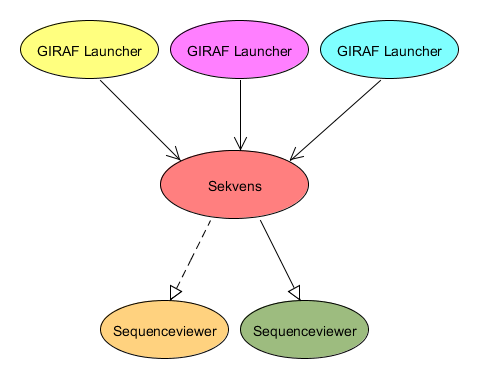
\includegraphics[scale=0.4]{Pics/sekvens.png}
	\caption{The position of Sekvens in the multi-project after Sprint 4.}
	\label{fig:sekvensContext}
\end{figure}
